\documentclass[french,a4paper,12pt]{report}
\usepackage[utf8]{inputenc}
\usepackage[T1]{fontenc}
\usepackage{graphicx}
\usepackage{float}
\usepackage{listings}
\usepackage{color}
\definecolor{dkgreen}{rgb}{0,0.6,0}
\definecolor{gray}{rgb}{0.5,0.5,0.5}
\definecolor{mauve}{rgb}{0.58,0,0.82}

\lstset{frame=tb,
  language=Java,
  aboveskip=3mm,
  belowskip=3mm,
  showstringspaces=false,
  columns=flexible,
  basicstyle={\small\ttfamily},
  numbers=none,
  numberstyle=\tiny\color{gray},
  keywordstyle=\color{blue},
  commentstyle=\color{dkgreen},
  stringstyle=\color{mauve},
  breaklines=true,
  breakatwhitespace=true,
  tabsize=3
}



\title{TR54 \\ TP Projet :\\ Intersection Autonome}
\author{Professeur encadrant :\\LOMBARD Alexandre \\\\ Élèves :\\ROMET Pierre\\Carrion Nicolas\\Burger Valentin\\Panassim Hessou}
%\hfill\hbox to 0pt{\hss\includegraphics[width=7cm]{Rapport_screen_activity-Stock_liste.png}\hss}\hfill\null\newline
\date{Automne 2017}

\begin{document}

\maketitle

\tableofcontents

\part{Introduction}
Lors de ce TP Projet,
il nous fut proposé d'implémenter des "Véhicules Guidés Autonome" (VGA), afin de mettre en œuvre un contrôle
temps réel sans fil, destiné à prévenir le passage d'une intersection selon un protocole prédéfini.

\part{Objectif}
L'objectif du projet est la réalisation d'une intersection autonome en utilisant les robots Légo EV3.
Trois robots (ou plus) devrons se déplacer sur un circuit en forme de huit et négocier leur droit de passage à
l'intersection par communication sans fil afin d'éviter les collisions.

\part{Éléments à notre disposition}
Afin de mettre en œuvre notre projet, nous avons eu à dispositions les éléments suivants.

\chapter{Le circuit}
Le circuit mise à notre disposition est découpé en plusieurs zones:
\begin{itemize}
\item Zone d’entrée/zone de stockage (approche de l’intersection)
\item Zone de conflit (où un seul robot peut être présent)
\item Zone de sortie
\end{itemize}

\hfill\hbox to 0pt{\hss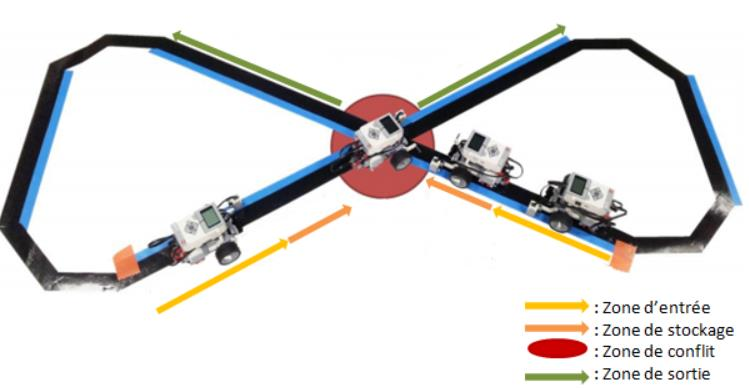
\includegraphics[width=15cm]{circuit.png}\hss}\hfill\null\newline

\chapter{Politique de négociation}
Afin de mettre en œuvre une régulation au sein de la zone d'intersection, quatre protocoles nous furent proposés
afin d'administrer le droit de passage.

\begin{itemize}
\item Feux communicants:
Programmation horaire en donnant la couleurs de feu à chaque voie (rouge/vert, rouge/rouge, vert/vert, vert/rouge).
On peut pousser l'approche pour que le robots soit au courant du temps qui reste pour obtenir le vert et ainsi adapter sa vitesse en fonction.

\item La négociation binaire:
Les véhicules arrivent et demande l'accès au serveur pour son passage.
Puis, si le passage n'est pas occupé, le robot obtient le droit de passage, sinon il est enregistré et il attend l'autorisation, qu'il aura une fois la zone libre.
Enfin, lorsque le robot à fini de traverser la zone, il envoie un acquittement, afin de notifier le serveur que la zone de conflit est libre.

\item Synchronisation de vitesse:
A l’approche de l’intersection (zone d’entrée) un robot envoie une requête de passage au serveur d’intersection.
De son côté le serveur construit une séquence de passage ordonnée à partir des requêtes reçues et la retransmet
à l’ensemble des robots concernés. La liste contient l’ensemble des robots ayant émis une requête pour franchir
l’intersection, leur position et leur vitesse. Tous les robots sont autorisés à franchir l’intersection, mais ils doivent synchroniser leur vitesse avec ceux qui les précèdent dans la séquence. Par exemple, si un robot est en position 3 dans la séquence, il ne pourra traverser qu’après que le robot en position 2 soit sorti de la séquence. Pour ce faire, chaque robot, une fois dans la séquence de passage, doit émettre régulièrement auprès du serveur des messages pour l’informer de sa nouvelle position et sa nouvelle vitesse. Ces informations sont retransmises à
tous les robots par la séquence de passage. Tant qu’un robot n’est pas dans la séquence de passage, il doit s’arrêter avant l’intersection.

\item Synchronisation par réservation (AIM):
Cette méthode fut développé par l'université du Texas, elle consiste à se que le véhicule estime l'horaire d'occupation de la zone de conflit afin de pouvoir demander une réservation.
Ainsi, si l'horaire est libre, le serveur l'accepte, sinon il lui refuse.
Enfin, en cas de refus, le véhicule devra retarder son horaire.
\end{itemize}

\chapter{Stratégie de régulation}
Concernant la construction de la séquence de passage, devant permettre le franchissement de la zone de conflit, deux stratégies nous furent proposées:

\begin{itemize}
\item FIFO (first-in first-out) : 
	Le premier arrivé à l’intersection est le premier à en sortir, dans le cadre de cette
	politique, un soin particulier devra être apporté à la prévention des situations d’inter-blocage
	
\item Batch : lorsqu’un robot se présente à l’intersection, il est ajouté à la séquence de passage, si et
	uniquement si, l’une des deux conditions suivantes est remplie :
	\begin{itemize}
	\item La séquence de passage actuelle est vide
	\item Le dernier robot dans la séquence de passage provient de la même voie que le robot actuel
	\item Le dernier robot dans la séquence de passage provient de l’autre voie, mais le délai entre l’ajout
		de ce dernier robot et du robot courant est supérieur à un seuil dT (par exemple 5 secondes)
	\end{itemize}
\end{itemize}

\part{Travail Réalisé}


\chapter{Intersection}

\section{Politique de négociation}

\section{Stratégie de régulation}

\chapter{Communication sans file}

\section{Serveur}%Valentin

\section{Client}%Pierre

\chapter{Le suivi de ligne} %Nico && Nadège

\part{Analyse critique}

\chapter{Difficultés rencontrées}

\chapter{Solutions apportées}

\part{Conclusion}


\end{document}
